%%%%%%%%%%%%%%%%%%%%%%%%%%%%%%%%%%%%%%%%%
% Beamer Presentation
% LaTeX Template
% Version 1.0 (10/11/12)
%
% This template has been downloaded from:
% http://www.LaTeXTemplates.com
%
% License:
% CC BY-NC-SA 3.0 (http://creativecommons.org/licenses/by-nc-sa/3.0/)
%
%%%%%%%%%%%%%%%%%%%%%%%%%%%%%%%%%%%%%%%%%

%----------------------------------------------------------------------------------------
%	PACKAGES AND THEMES
%----------------------------------------------------------------------------------------

\documentclass[9pt]{beamer}
\usepackage{CJK}
\usepackage{ctex}
\usepackage{graphicx}
\usepackage{subfigure}
\usepackage{longtable}
\usepackage{rotating}
\usepackage{multirow}
\usepackage{algorithm}
\usepackage{algorithmic}
\usepackage{mathtools}
\usepackage{animate}
\usepackage{amsthm, amsmath}
%\usepackage{media9}
%% A LATEX package for embedding interactive Adobe Flash (SWF) and 3D files (Adobe U3D & PRC) as well as video and sound files or streams (FLV, MP4/H.246, MP3) into PDF documents with Adobe Reader-9/X
%compatibility.
\renewcommand{\algorithmicrequire}{\textbf{Input:}}   %Use Input in the format of Algorithm
\renewcommand{\algorithmicensure}{\textbf{Output:}}  %UseOutput in the format of Algorithm
\newcommand{\e}[1]{\ensuremath{\times 10^{#1}}}
%\mode<presentation>{\usetheme{Madrid}}

\mode<presentation> {

% The Beamer class comes with a number of default slide themes
% which change the colors and layouts of slides. Below this is a list
% of all the themes, uncomment each in turn to see what they look like.

%\usetheme{default}
%\usetheme{AnnArbor}
%\usetheme{Antibes}
%\usetheme{Bergen}
%\usetheme{Berkeley}
%\usetheme{Berlin}
%\usetheme{Boadilla}
%\usetheme{CambridgeUS}
%\usetheme{Copenhagen}
%\usetheme{Darmstadt}
%\usetheme{Dresden}
%\usetheme{Frankfurt}
%\usetheme{Goettingen}
%\usetheme{Hannover}
%\usetheme{Ilmenau}
%\usetheme{JuanLesPins}
%\usetheme{Luebeck}
\usetheme{Madrid}
%\usetheme{Malmoe}
%\usetheme{Marburg}
%\usetheme{Montpellier}
%\usetheme{PaloAlto}
%\usetheme{Pittsburgh}
%\usetheme{Rochester}
%\usetheme{Singapore}
%\usetheme{Szeged}
%\usetheme{Warsaw}

% As well as themes, the Beamer class has a number of color themes
% for any slide theme. Uncomment each of these in turn to see how it
% changes the colors of your current slide theme.

%\usecolortheme{albatross}
\usecolortheme{beaver}
%\usecolortheme{beetle}
%\usecolortheme{crane}
%\usecolortheme{dolphin}
%\usecolortheme{dove}
%\usecolortheme{fly}
%\usecolortheme{lily}
%\usecolortheme{orchid}
%\usecolortheme{rose}
%\usecolortheme{seagull}
%\usecolortheme{seahorse}
%\usecolortheme{whale}
%\usecolortheme{wolverine}

%\setbeamertemplate{footline} % To remove the footer line in all slides uncomment this line
%\setbeamertemplate{footline}[page number] % To replace the footer line in all slides with a simple slide count uncomment this line

%\setbeamertemplate{navigation symbols}{} % To remove the navigation symbols from the bottom of all slides uncomment this line
}

\renewcommand{\algorithmicrequire}{\textbf{Input:}}   %Use Input in the format of Algorithm
\renewcommand{\algorithmicensure}{\textbf{Output:}}  %UseOutput in the format of Algorithm

%\mode<presentation>{\usetheme{Madrid}}

\usepackage{graphicx} % Allows including images
\usepackage{booktabs} % Allows the use of \toprule, \midrule and \bottomrule in tables
\begin{document}
\begin{CJK*}{GBK}{kai}
%----------------------------------------------------------------------------------------
%	TITLE PAGE
%----------------------------------------------------------------------------------------

\title[Machine Learning]{Gradient Descent (and beyond)} % The short title appears at the bottom of every slide, the full title is only on the title page

\author{Kun He (����)} % Your name
%\logo{%
%   
\includegraphics[scale=.2]{logo.pdf}\hspace*{4.75cm}~%
%   
\includegraphics[scale=.2]{logo.jpg}\hspace*{0.75cm}%
%   }
%\pgfdeclareimage[width=1cm]{hust}{logo.pdf}
%\logo{\pgfuseimage{hust}{\vspace{-10pt}}}
\titlegraphic{
\includegraphics[width=1.3cm]{logo.pdf}}
\institute[JHL, HUST] % Your institution as it will appear on the bottom of every slide, may be shorthand to save space
{
	Data Mining and Machine Learning Lab\\
	(John Hopcroft Lab)\\
	Huazhong University of Science \& Technology \\ % Your institution for the title page
	\medskip
	\textit{brooklet60@hust.edu.cn} % Your email address
}

\date{2022��5��} % Date, can be changed to a custom date
%====================================================
\frame{\titlepage}

\frame{\frametitle{Table of contents}\tableofcontents}

\AtBeginSection[]
{
\begin{frame}{Table of Contents}
\tableofcontents[currentsection]
\end{frame}
}

%------------------------------------------------
%------------------------------------------------

\section{Introduction}
%------------------------------------------------
\subsection{Review}
\begin{frame}
	\frametitle{Review}
\begin{itemize}
	\item In the previous lecture on Logistic Regression we wrote down expressions for the parameters in our model as solutions to optimization problems that do not have closed form solutions. 
	\item Specifically, given data 
$\{(x_i,y_i)\}_ {i=1}^n$
with $x_i\in\mathbb{R}^d$ and $y_i\in\{+1,-1\}$
we saw that
\end{itemize}
	\[\hat{w}_{\text{MLE}} = \mathop{\mathrm{arg\,min}}_{w\in\mathbb{R}^d,b\in\mathbb{R}}\; \sum_{i=1}^n \log(1+e^{-y_i(w^Tx_i+b)})
	\]
~~~~~~~~~~	and 
	\[
	\hat{w}_{\text{MAP}} = \mathop{\mathrm{arg\,min}}_{w\in\mathbb{R}^d,b\in\mathbb{R}}\; \sum_{i=1}^n \log(1+e^{-y_i(w^Tx_i+b)}) + \lambda w^Tw.
	\]
\begin{itemize}
	\item These notes will discuss general strategies to solve these problems and, therefore, we abstract our problem to
\end{itemize}	
	\[\min_{w} \ell(w)\]
~~~~~~~~~~	where $\ell\colon \mathbb{R}^d \rightarrow \mathbb{R}$. 
	
 
\end{frame}
%------------------------------------------------
 
\begin{frame}
\frametitle{Review}
While we will discuss some basic algorithmic strategies here.\\
	
We want to minimize a \textbf{convex}, \textbf{continuous} and \textbf{differentiable} loss function $\ell(w)$. 

\begin{itemize}
	\item $\ell$ is convex. This allows us to assert that any local minimum we find is also a global minimum, and helps simplify our discussion of Newton��s method.
	\item $\ell$ is at least thrice continuously differentiable. We are going to extensively use Taylor approximations and this assumption simplifies the discussion greatly.
	\item There are no constraints placed on $w$.  Adding constraints is a level of complexity we will not address here.
\end{itemize}	
In this section we discuss two of the most popular "hill-climbing" algorithms, gradient descent and Newton's method
for $\min_{w} \ell(w)$.

\end{frame}
%------------------------------------------------
\subsection{Local minimizer}
\begin{frame}
\frametitle{What is a (local) minimizer}
\begin{itemize}
\item The first question we might ask is what it actually means to solve $\min_{w} \ell(w)$. We call $w^*$
a local minimizer of $\ell$ if:
\end{itemize}
\begin{block}{Local minimizer:}
	There is some $\epsilon > 0$ such that for $\{w \,\vert\, \|w-w^*\|_ 2 < \epsilon\}$ we have that $\ell(w^*) \leq \ell(w ).$
\end{block} 

\begin{itemize}
	\item Our earlier assumption that $\ell$  is convex implies that if we find such a $w^*$ we can immediately assert that $\ell(w^*) \leq \ell(w)$
	for all $w\in\mathbb{R}^d.$
	\item we can also define a strict local minimizer by forcing $\ell(w^*) < \ell(w).$
	\item Notably, some convex functions have no strict local minimizers, e.g., the constant function $\ell(w) = 1$ is convex.
	\item Some convex functions have no finite local minimizers, e.g., for any non-zero vector $c\in\mathbb{R}^d$, 
	$c^Tw$ is convex but can be made arbitrarily small by letting  appropriately.
	\item A key necessary condition for a point to be a local minimizer is that the gradient of $\ell$ is zero at $w^*$, 
	i.e., $\nabla\ell(w^*) = 0.$
	\item Assuming the gradient at $w^*$
	is zero, a sufficient condition for the point to be a strict local minimizer is for the Hessian, i.e., $\nabla^2\ell(w^*)$
	to be positive definite.
	
\end{itemize}
\end{frame}
%------------------------------------------------
\section{Taylor Expansions}
\subsection{Taylor expansions}
\begin{frame}
	\frametitle{Taylor expansions}
	\begin{itemize}
	\item While we made some assumptions on $\ell$ they do not actually tell us much about the function��it could behave in all sorts of ways. Moreover, as motivated by the logistic regression example it may not be so easy to work with the function globally. 
	\item Therefore, we will often leverage local information about the function $\ell$. We accomplish this through the use of first and second order Taylor expansions. 
	\end{itemize}
\end{frame}

%------------------------------------------------
\begin{frame}
	\frametitle{Taylor expansions}
\begin{block}{First order Taylor expansion}
The first order Taylor expansion of  centered at  can be written as
\[ \ell(w+p) \approx \ell(w) + g(w)^Tp,
\]
where $g(w)$ is the gradient of $\ell$ evaluated at $w$ i.e., $(g(w))_ j = \frac{\partial \ell}{\partial w_j}(w)$
for $j=1,\ldots,d.$
\end{block} 

\begin{block}{Second order Taylor expansion}
	The second order Taylor expansion of  centered at $\ell$ can be written as
	\[  \ell(w+p) \approx \ell(w) + g(w)^Tp + \frac{1}{2}p^T H(w)p ,
	\]
	where  $H(w)$ is the Hessian of $\ell$ evaluated at $w$, i.e., 
	\[
	[H(w)]_ {i,j} = \frac{\partial^2 \ell}{\partial w_i\partial w_j}(w) \]
	for $j=1,\ldots,d.$
\end{block} 
 
\end{frame}

%------------------------------------------------
\subsection{First and second order Taylor approximations}
\begin{frame}
	\frametitle{First and second order Taylor approximations}
	\begin{itemize}
		\item These correspond to linear and quadratic approximations of $\ell$.
		\item In general, these approximations are reasonably valid if $p$ is small (concretely, first order has error $\mathcal{O}(\|p\|_ 2^2)$
		and second order has error $\mathcal{O}(\|p\|_ 2^3)$
		).
	\end{itemize}
~~
\begin{figure}[h]
	\centering
	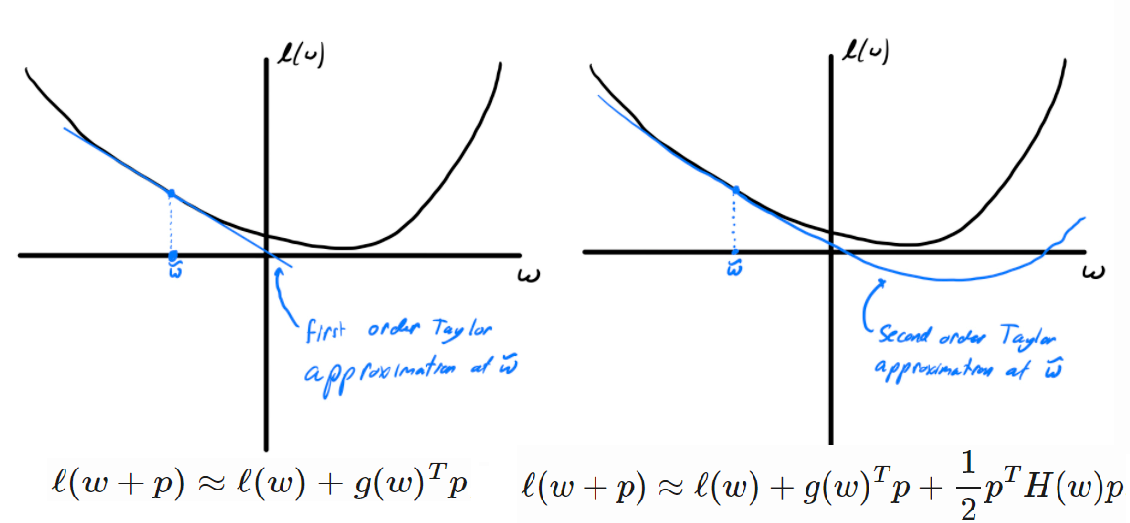
\includegraphics[scale=0.4]{TaylorApproximation}
\end{figure}
\end{frame}

%------------------------------------------------
\section{Search Direction Methods}
%------------------------------------------------
%\subsection{Search direction methods}
\begin{frame}
	\frametitle{Search direction methods}
	\begin{block}{Loss function}
		\[\min_{w} \ell(w),\] 
	\end{block}
	\begin{itemize}
	\item The core idea is that given a  starting point $w^0$ we construct a sequence of iterates $w^1,w^2,\ldots$ with the goal that $w^k\rightarrow w^*$ as $k\rightarrow \infty.$
	\item In a search direction method we will think of constructing $w^{k+1}$ from $w^{k}$ by writing it as $w^{k+1} = w^{k} + s$ for some ��step�� $s$. 
    \end{itemize}
\begin{figure}[h]
	\centering
	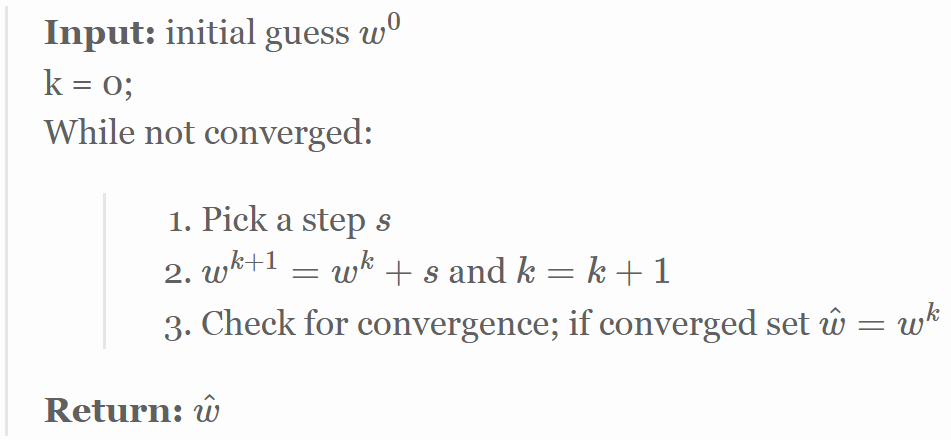
\includegraphics[scale=0.25]{GDalgo.png}
	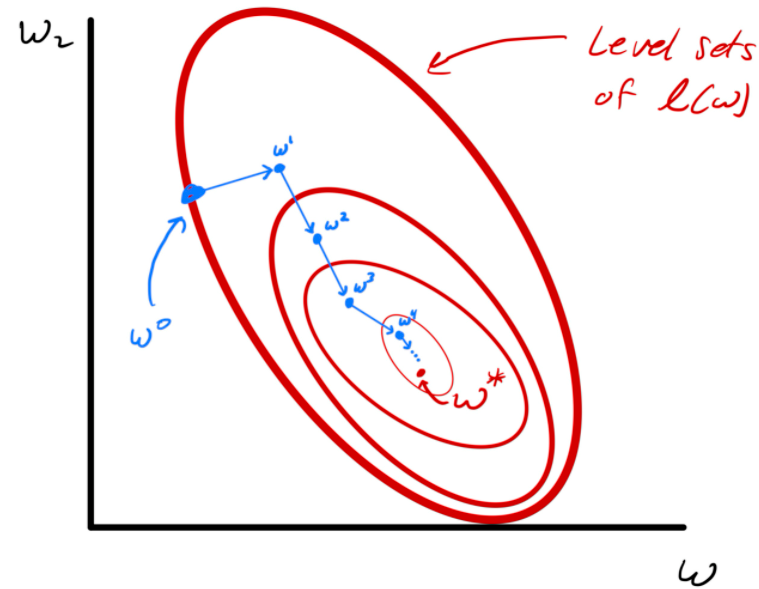
\includegraphics[scale=0.25]{SearchDirectionMethod.png}	
	
\end{figure}

\end{frame}
%------------------------------------------------
%\subsection{methods}
\begin{frame}
	\frametitle{Search direction methods}
	\begin{block}{Two key steps}
	There are two clearly ambiguous steps in the above algorithm:
	\begin{itemize}
	\item \textbf{How do we pick $s$}.  
	\item how do we determine when we have converged.  
	\end{itemize}
	\end{block}	
We will spend most of our time addressing the former and then briefly touch on the latter��robustly determining convergence is one of the little details that a good optimization package should do well.
\end{frame}

%------------------------------------------------
\section{Gradient Descent}
%------------------------------------------------
%\subsection{Gradient descent}
\begin{frame}
	\frametitle{Gradient descent}
	\begin{block}{Core idea}
		Given we are currently at 
		determine the direction in which the function decreases the fastest (at this point) and take a step in that direction. 
	\end{block}
Considering the linear approximation to  at 
	provided by the Taylor series    
 
     \[\ell(w^k +s) = \ell(w^k) + g(w^k)^Ts\]
then the fastest direction to descend is simply $s \propto -g(w^k)$. \\

what we actually do in gradient descent is set $s$ as
	\[s = -\alpha g(w^k)\]
for some step size $\alpha > 0$.	

\end{frame}

%------------------------------------------------
%\subsection{methods}
\begin{frame}
	\frametitle{Gradient descent}
	\begin{block}{Correctness}
		There is always some small enough $\alpha$ such that
		\[\ell(w^k-\alpha g(w^k)) < \ell(w^k).\]
	\end{block}
	Question: Why? 
	\[\ell(w^k +s) = \ell(w^k) + g(w^k)^Ts\]
	\[s = -\alpha g(w^k)\]
	\[\alpha > 0\]
\end{frame}


 
%------------------------------------------------
%\subsection{methods}
\begin{frame}
	\frametitle{Gradient descent}
	\begin{block}{Correctness}
		There is always some small enough $\alpha$ such that
		\[\ell(w^k-\alpha g(w^k)) < \ell(w^k).\]
	\end{block}
	\[ \ell(w^k-\alpha g(w^k)) = \ell(w^k) - \alpha g(w^k)^Tg(w^k) + \mathcal{O}(\alpha^2).\]
	Since 
	\[g(w^k)^Tg(w^k) > 0\]
	and 
	$\alpha^2 \rightarrow 0$ faster than $\alpha$ as $\alpha\rightarrow 0$.\\
	We conclude that for some sufficiently small $\alpha > 0$ we have that $\ell(w^k-\alpha g(w^k)) < \ell(w^k).$
	
\end{frame}

%------------------------------------------------
%\subsection{methods}
\begin{frame}
	\frametitle{Determine the step size}
	\begin{itemize}
		\item  In classical optimization, $\alpha$ is often referred to as the step size (in this case $g(w^{k})$ is the search direction).  
		\item However, they can be more expensive then a fixed strategy for setting $\alpha$.  The catch is that setting $\alpha$ too small can lead to slow convergence and setting $\alpha$ too large can actually lead to divergence.  
	\end{itemize}

\begin{figure}[h]
	\centering
	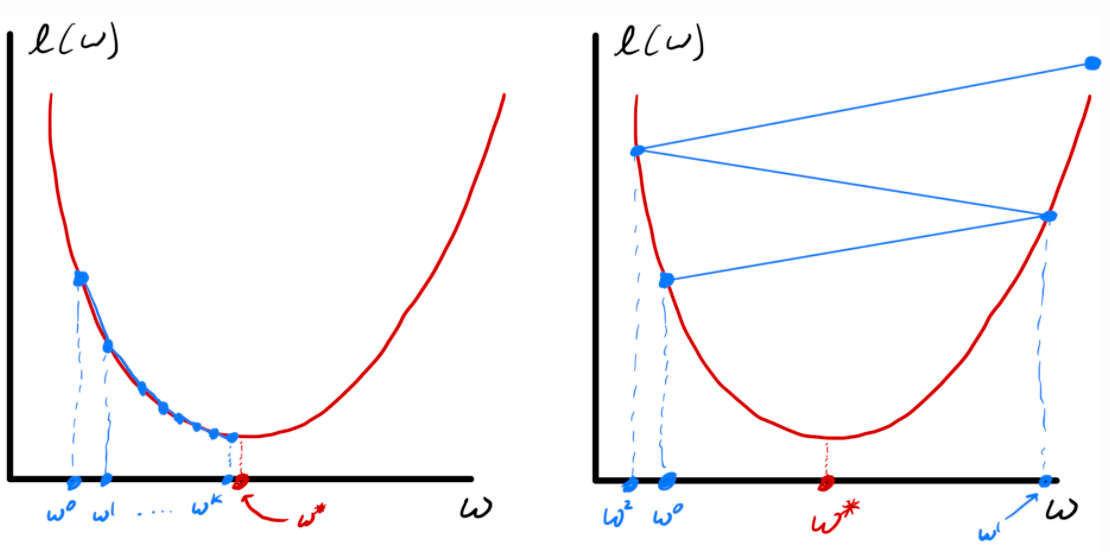
\includegraphics[scale=0.3]{StepSize.png}
	\caption{Choices of the step size that lead to convergence (left) or divergence (right).}
\end{figure}
\end{frame}

%------------------------------------------------
\section{Adagrad}
%------------------------------------------------
%\subsection{methods}
\begin{frame}
	\frametitle{Adagrad}
	\begin{itemize}
		\item One option is to set the step-size adaptively for every feature.  
		\item Adagrad accomplishes this by keeping a running average of the squared gradient with respect to each optimization variable.
		\item It then sets a small learning rate for variables with large gradients and a large learning rate for features with small gradients.
		\item This can be important if the entries of $w$ are attached to features (e.g., in logistic regression we can associate each entry of  $w$ with a feature) that vary in scale or frequency. 
	\end{itemize}	
\end{frame}
%------------------------------------------------
%\subsection{methods}
\begin{frame}
	\frametitle{Adagrad}
 	\begin{figure}[h]
 	\centering
 	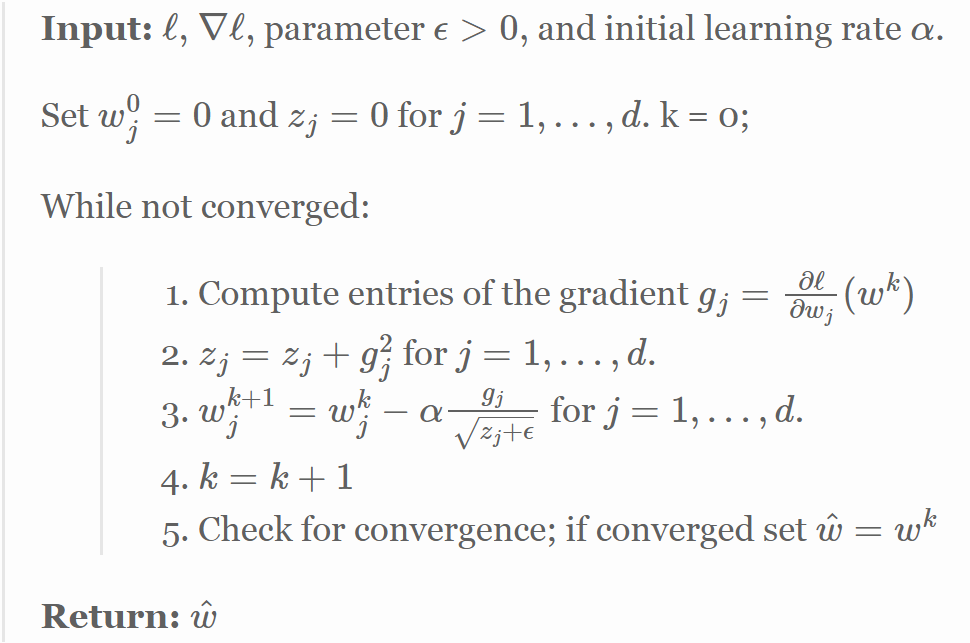
\includegraphics[scale=0.35]{Adagrad.png}
 	\end{figure}	
 \textbf{Keypoint}: Every dimension uses its own learning rate.
 \\
 \textbf{Question}: Why add $\epsilon$?
\end{frame}

%------------------------------------------------
\section{Newton's method}
%------------------------------------------------
%\subsection{methods}
\begin{frame}
	\frametitle{Newton's method}
	\begin{block}{Core idea}
		Use second order information (quadratic approximation). 
		\[\ell(w^k+s) \approx \ell(w^k) + g(w^k)^Ts + \frac{1}{2}s^T H(w^k)s.\]
	\end{block}
	\begin{itemize}
		\item  We now chose a step by explicitly minimizing the quadratic approximation to $\ell$ at $w^k$.
		\item Recall that because $\ell$ is convex $H(w)$ is positive semi-definite for all $w$ so this is a sensible thing to attempt.  
		\item In fact, Newton's method has very good properties in the neighborhood of a strict local minimizer and once close enough to a solution it converges rapidly.
	\end{itemize}
\begin{figure}[h]
	\centering
	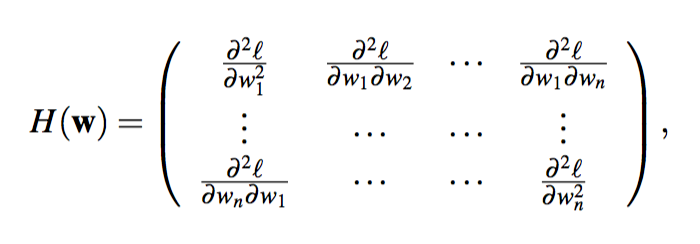
\includegraphics[scale=0.4]{HessianMatrix}
\end{figure}	
\end{frame}

%------------------------------------------------
%\subsection{methods}
\begin{frame}
	\frametitle{Newton's method}
	\begin{block}{Core idea}
		Use second order information (quadratic approximation). 
		\[\ell(w^k+s) \approx \ell(w^k) + g(w^k)^Ts + \frac{1}{2}s^T H(w^k)s.\]
	\end{block}
	\begin{itemize}
		\item  For simplicity, lets assume  that $H(w^k)$ is positive definite.
		\item The gradient of our quadratic approximation is $g(w^k)+H(w^k)s$.
		\item This implies that $s$ solves the linear system:  
	\end{itemize}	
	\[ H(w^k)s = -g(w^k).
	\]
	\[~~~~~~~~~~ s = - H^{-1}(w^k)g(w^k).
\]
	
\end{frame}
%------------------------------------------------
\section{A Simple Example}
%------------------------------------------------
%\subsection{methods}
\begin{frame}
	\frametitle{A simple example}
	\begin{block}{}
	\begin{itemize}
		\item There is a simple example that clearly illustrates how incorporating second order information can help. 
		\item Pretend the function  was actually a strictly convex quadratic, i.e.,  
	\end{itemize}	
	\[
	\ell(w) = \frac{1}{2}w^TAw + b^Tw + c
	\]
	where $A$ is a positive definite matrix, $b$ is an arbitrary vector, and $c$ is some number.
	\end{block}
	\textbf{Question}: How many steps does Newton converge?  
\end{frame}

%------------------------------------------------
\begin{frame}
	\frametitle{A simple example}
	\begin{block}{}
	\begin{itemize}
		\item Pretend the function  was actually a strictly convex quadratic, i.e.,  
	\end{itemize}	
	\[
	\ell(w) = \frac{1}{2}w^TAw + b^Tw + c
	\]
	where $A$ is a positive definite matrix, $b$ is an arbitrary vector, and $c$ is some number.
    \end{block}
	In this case, Newton converges in one step (since the strict global minimizer 
	of $w^*$ is the unique solution to $Aw = b$).
\end{frame}

%------------------------------------------------
\begin{frame}
	\frametitle{A simple example}

	\begin{block}{}
	\begin{itemize}
		\item Pretend the function  was actually a strictly convex quadratic, i.e.,  
	\end{itemize}	
	\[
	\ell(w) = \frac{1}{2}w^TAw + b^Tw + c
	\]
	where $A$ is a positive definite matrix, $b$ is an arbitrary vector, and $c$ is some number.
	\end{block}

	Meanwhile, gradient descent yields the sequence of iterates
	\[ w^{k} = (I - \alpha A)w^{k-1} - \alpha b.
	\]
	Using the fact that $w^*= (I-\alpha A)w^*- \alpha b$ we can see that 
	\begin{align}
	\|w^{k} - w^*\| &\leq \|I - \alpha A\|_ 2 \|w^{k-1} - w^*\|_ 2 \\
	&\leq \|I - \alpha A\|_ 2^k \|w^{0} - w^*\|_ 2.
	\end{align}
\end{frame}

%------------------------------------------------
\begin{frame}
	\frametitle{A simple example}
	\begin{itemize}
		\item  Therefore, as long as $\alpha$ is small enough such that all the eigenvalues of $I - \alpha A$ are in (-1,1), the iteration will converge��albeit slowly if we have eigenvalues close to $\pm 1$.  
		\item  More generally, fig. 4 shows an example where we see the accelerated convergence of Newton��s method as we approach the local minimizer.  
	\end{itemize}	
	The following figure shows an example where we see the accelerated convergence of Newton's method as we approach the local minimizer.
	\begin{figure}[h]
		\centering
		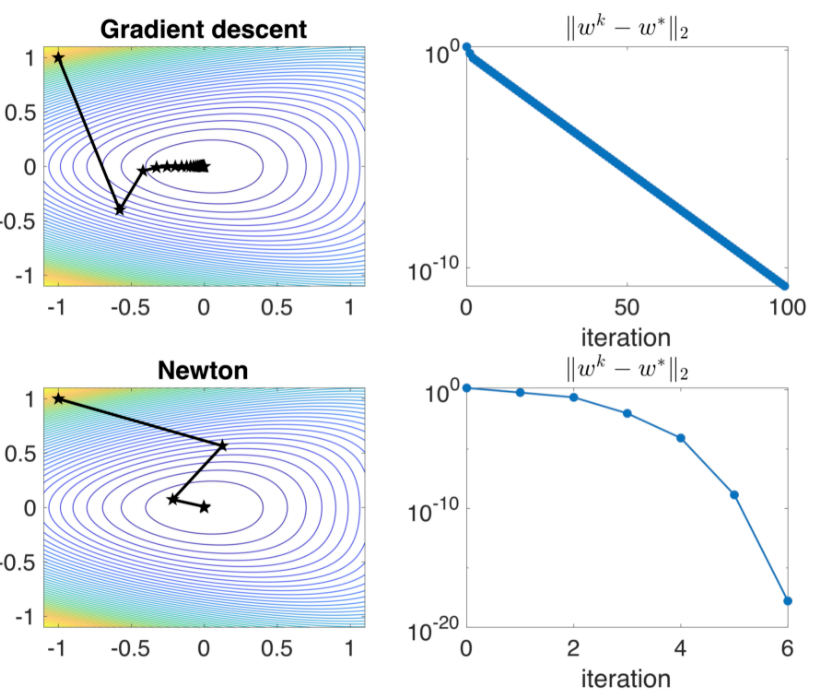
\includegraphics[scale=0.3]{Newton.png}
	\end{figure} 
	
\end{frame}
%------------------------------------------------
\section{Best Practices}
%------------------------------------------------
%\subsection{methods}
\begin{frame}
	\frametitle{Best Practices}
	\begin{itemize}
		\item  The matrix $H(w)$ scales $d \times d$ and is expensive to compute. A good approximation can be to \textbf{only compute its diagonal entries and multiply the update with a small step-size}. Essentially you are then doing a hybrid between Newton's method and gradient descent, where you weigh the step-size for each dimension by the inverse Hessian..  
		\item To avoid divergence of Newton's method, a good approach is to \textbf{start with gradient descent (or even stochastic gradient descent) and then finish the optimization Newton's method}. Typically, the second order approximation, used by Newton's Method, is more likely to be appropriate near the optimum.  
	\end{itemize}	
\end{frame}
%------------------------------------------------
\iffalse
\section{methods}
%------------------------------------------------
%\subsection{methods}
\begin{frame}
	\frametitle{methods}
	\begin{block}{Core idea}
		Use second order information
	\end{block}
	\begin{itemize}
	\item  How  .  
	\item how .  
	\end{itemize}	
\end{frame}
\fi
%------------------------------------------------

%------------------------------------------------

 


%%------------------------------------------------
%\section{Reference}
%------------------------------------------------
%\begin{frame}
%\frametitle{Reference}
%\begin{thebibliography}{4}
%\bibitem{LS-SPH} F. Zou, C. Liu, H. Ling, H. Feng, L. Yan, and D. Li, "Least square regularized spectral hashing for similarity search," Signal Processing, vol. 93, pp. 2265-2273, 2013. (SCI,EI)
%\bibitem{KMFH} F. Zou, Y. Chen, J. Song, K. Zhou, Y. Yang, and N. Sebe, "Compact image fingerprint via multiple kernel hashing," IEEE Transactions on Multimedia, vol. 17, pp. 1006-1018, 2015. (SCI,EI)
%\bibitem{KNPH} C. Liu, H. Ling, F. Zou, L. Yan, Y. Wang, H. Feng, et al., "Kernelized neighborhood preserving hashing for social-network-oriented digital fingerprints," IEEE Transactions on Information Forensics and Security, vol. 9, pp. 2232-2247, 2014. (SCI,EI)
%\bibitem{DTSH} Liu, Yu; Song, Jingkuan; Zhou, Ke; Yan, Lingyu; Liu, Li; Zou, Fuhao; Shao, Ling, "Deep Self-taught Hashing for Image Retrieval," IEEE Tra
%\bibitem{DeepFace} Fuhao Zou, Fan Yang, Wei Chen,Kai Lia, Jingkuan Song, Jingcai Chen, Hefei Ling, "Fast Large Scale Deep Face Search," Pattern Recognition Letters, Januray 3, 2019. (SCI,EI)
%\end{thebibliography}
%\end{frame}
%------------------------------------------------
\begin{frame}
\Huge{\centerline{The End}}
\end{frame}

\end{CJK*}
\end{document}
%\end{document}
